\section{Visual Object Tracking Benchmark}
\label{sec:tracking}
In visual object tracking, a drone follows a moving target and tries
to keep it centered in its FOV.  Many surveillance-related instances
of this task, where the target may be adversarial and actively try to
escape tracking, occur in law enforcement and military settings.  The
task is also relevant to wildlife conservation research, where an
animal of an endangered species is identified and followed in the
wild.  It is also used in filmmaking to capture evolving scenes.  In
such use cases, using an autonomous drone for tracking could reduce
attention demand on mission personnel.

\subsection{Benchmark Requirements}
\label{sec:tracking-requirements}

A good benchmark for a task must capture the essential characteristics of successful completion. The size and visual appearance of a target plays an important role in
tracking success.  An object that is just a few pixels in size from
the altitude of the drone will be inherently difficult to
detect~\cite{Huang2017}.  Poor contrast with the background, as
happens when camouflaged, also contributes to poor detection.  Objects
that are hard to detect are also hard to track, since actuating to
re-center the target in each frame is key to success.  The object
being tracked and the background on which it moves both need to be
specified.  Only when these factors and drone optics are held
constant will \ooda~loop performance come to the fore in determining
tracking performance.

The benchmark should also be parameterized, so that it is easy to
vary the difficulty of the benchmark.  The benchmark should only use
standardized, off-the-shelf components that can be easily purchased or
fabricated.  There should be no ambiguity in the experimental setup or
interpretation of results, thereby simplifying independent attempts to
reproduce published experimental results.

\subsection{Benchmark Description}
\label{sec:tracking-description}
The object followed in my tracking benchmark is a DJI Robomaster S1
robot~\cite{Robomaster2022} as in Section~\ref{sec:task3}.  Tracking is done on a level, green background such as a football field.  For this combination of target and background, DNN-based object detection from an altitude of 10~m is successful at a confidence level of 0.9 or higher on frames from my drone's video camera.

My benchmark is a random walk with turns in a randomly-chosen
cardinal direction at each step.  Figure~\ref{fig:tracking-path}(a)
shows one example with 5 steps, and Figure~\ref{fig:tracking-path}(b)
shows other examples with more steps.  The benchmark has three
parameters: the number of steps;  the mean length of each step;
and the target speed of 1.5~m/s, 2.5~m/s, or 3.5~m/s.  The
benchmark could be made more complex by making the turns to be at any
angle rather than just cardinal directions, and by making step size
and target speed non-uniform.  All my experiments were conducted
across the full range of speeds, using a stepcount of 35 steps
and stepsize  set to 5~m.

\begin{figure}
\centering
\begin{minipage}{0.6\linewidth}
\centering
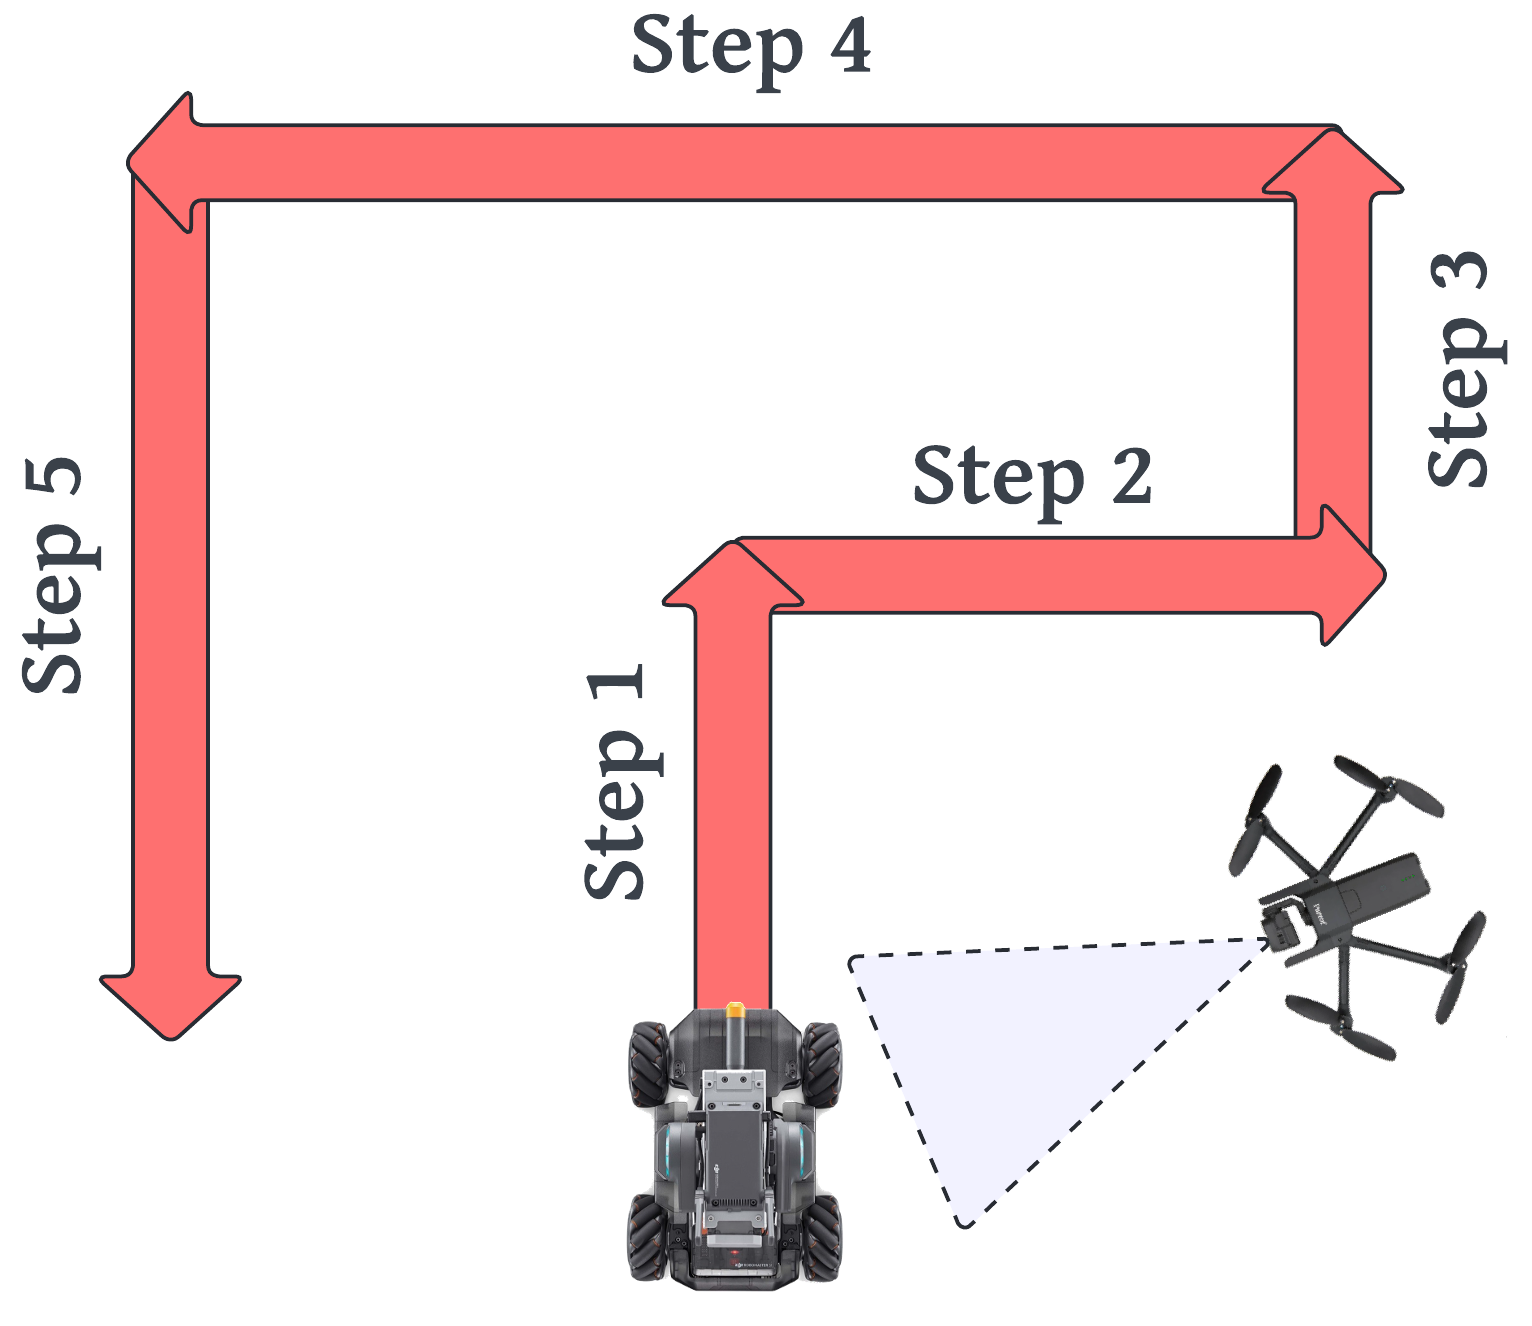
\includegraphics[width=0.8\linewidth]{chapter6/FIGS/fig-tracking-onepath.png}\\
{(a) Detail for 5-Step Example}
\end{minipage}
\begin{minipage}{0.35\linewidth}
\centering
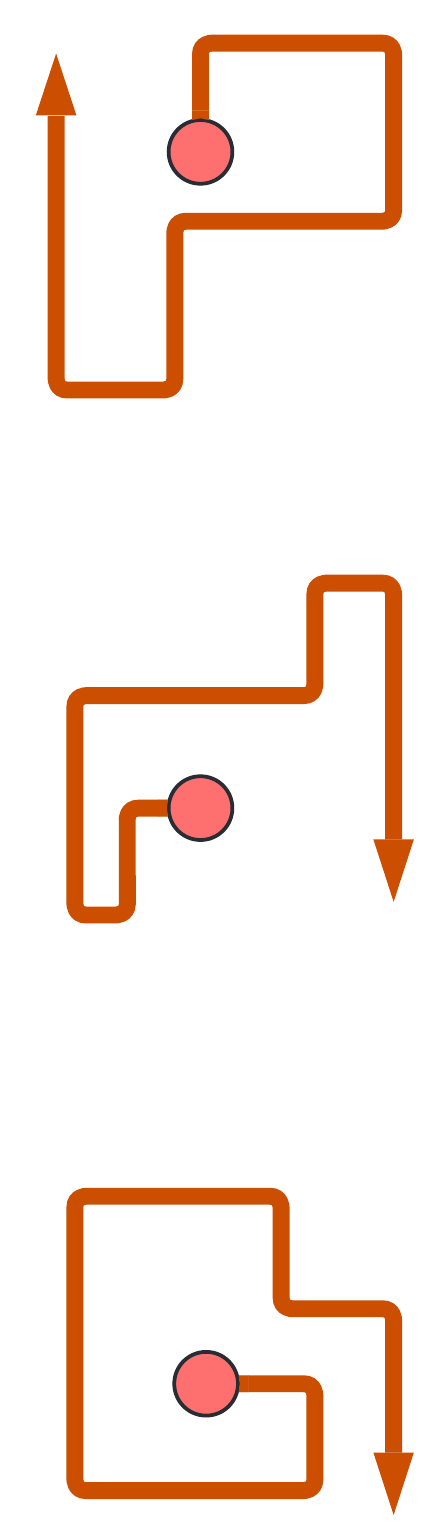
\includegraphics[width=0.35\linewidth]{chapter6/FIGS/fig-tracking-manypaths.png}\\
{(b) Other Examples}

\end{minipage}
\caption{Parameterized Random Walk}
\label{fig:tracking-path}
\end{figure}


To execute the benchmark, the target is placed in a large open outdoor
area.  The drone is manually piloted to the desired altitude, and its
FOV is adjusted to center the target. Once the drone has locked
onto its target, the target is instructed to start its pre-programmed
random walk and a timekeeper starts a stopwatch. The experiment
continues until one minute has elapsed or the drone loses the target
from its FOV.  The termination time and the black box footage of the
flight are logged for post-flight
scoring~(\S\ref{sec:tracking-scoring}).

\begin{figure}
\centering
\begin{minipage}{0.35\linewidth}
\centering
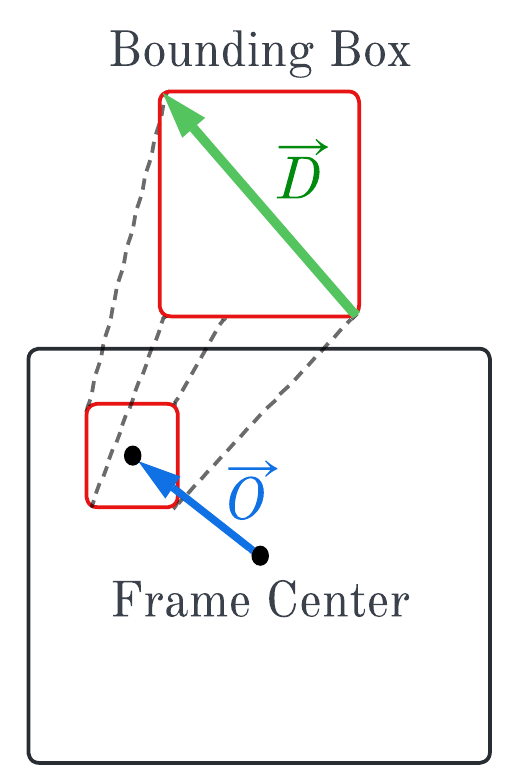
\includegraphics[width=\linewidth]{chapter6/FIGS/fig-tracking-scoring.png}
\caption{\small $\vec{O}$ \& $\vec{D}$}
\label{fig:o-d-calc}
\end{minipage}
\begin{minipage}{0.5\linewidth}
\small
\begin{equation}
	c_i = \norm{\vec{O}_i} / \norm{\vec{D}_i}\label{eq:2}
\end{equation}
\begin{equation}
	s_{i} = 1.1^{-c_i}\label{eq:3}
\end{equation}
\begin{equation}
	s_{\text{avg}} = \frac{\Sigma_i^n s_i}{n}\label{eq:4}
\end{equation}
\caption{Calculating Score}
{\centering\small\\[0.2cm]
$\norm{\vec{O}} = 0.11$, $\norm{\vec{D}} = 0.03$, $c = 3.67$ \\[0.1in]
$s_{10} = 1.1^{-c} = 0.70$ \\
$s_{20} = 1.2^{-c} = 0.51$ \\
$s_{30} = 1.3^{-c} = 0.38$ \\
}
\caption{Scoring Figure~\ref{fig:track-score-example}}
\label{fig:example-score-calcuclation}
\end{minipage}
\end{figure}

\begin{figure}
\centering
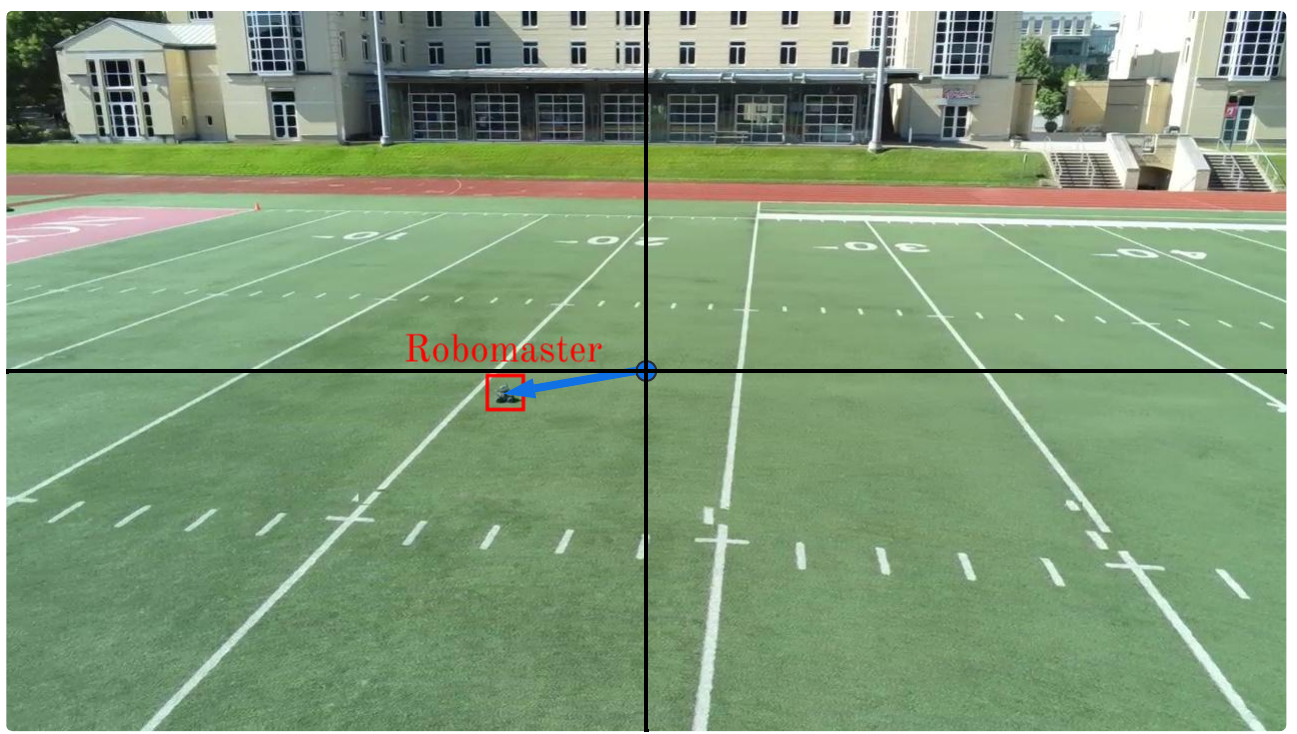
\includegraphics[width=0.9\linewidth]{chapter6/FIGS/fig-tracking-score-demo.png}
\caption{Example Frame for Scoring}
\label{fig:track-score-example}
\end{figure}

\subsection{Benchmark Scoring}
\label{sec:tracking-scoring}
In post-processing after a flight, I score the recorded video footage
using an automated process.  Figures~\ref{fig:o-d-calc} to
\ref{fig:example-score-calcuclation} show the scoring calculation,
using Figure~\ref{fig:track-score-example} as an example.  On each
frame, a DNN is first used to create a bounding box around the target.
With the center of the frame as the origin, the relative distance of
the target from the origin is obtained.  Using the notation shown in
Figure~\ref{fig:o-d-calc}, the pixel offset vector, $\vec{O}$, gives
the L2 distance of the target's centroid from the origin.  This is scaled
to the diagonal length of the bounding box, $\vec{D}$, to give the
centering ratio $c_i$~(formula \ref{eq:2}).  I then calculate the
score of the frame, $s_i$, by using an inverse exponential, as shown
in formula~\ref{eq:3}.  The rationale for using an exponential is to
super-linearly penalize distance from origin.  I use a compounding
10\% penalty in reporting my results, leading to the value of 1.1 in
formula~\ref{eq:3}.  Using $s_n$ to denote a penalty of n\%,
Figure~\ref{fig:example-score-calcuclation} shows the scores for
penalties of 10\%, 20\% and 30\% for the example frame in
Figure~\ref{fig:track-score-example}.  A score of zero is awarded when
the frame does not contain the target at all, or if the target is too
small to be detected in post-processing by a specified model.  In my
case, this model is YOLOv5x trained on aerial images of the target. This scoring is meant to award high scores to targets that are centered in frame but take up most of the frame real estate.

From the per-frame scores, the entire flight is scored by simple
averaging ~(formula \ref{eq:4}). The overall score, $s_{\text{avg}}$,
lies between $0$ and $1$, with higher being better. For
example, an average score of $0.70$ based on $s_{10}$ is achieved when
the drone is able to keep the target within about three normalized
lengths of the center of the FOV for the entire duration of the
flight.

\begin{table}
\centering
\begin{tabular}{|l|c|c|c|}
\hline
\textbf{Model} & \textbf{Latency} & \textbf{Throughput} & \textbf{mAP} \\
 & (ms) & (fps) & \\
\hline
YOLOv5s  & 28 & 25 & 56.8\\
YOLOv5m  & 37 & 20 & 64.1\\
YOLOv5l  & 42 & 20 & 67.3\\
\hline
\end{tabular}
\begin{captext}
  \\[0.1cm] \small The inference and throughput were obtained on the
  cloudlet~(\S\ref{sec:cloudlet}).  The mean average precision~(mAP)
  is from the YOLO documentation~\cite{Yolo}.
\end{captext}
\caption{YOLOv5 Performance in the SteelEagle Pipeline}
\label{fig:yolo-model-stats}
\end{table}


\subsection{Tracking Algorithm}
\label{sec:tracking-algorithm}
For this benchmark, I use the tracking algorithm used described in Section~\ref{sec:tracking-algorithm-advanced}. Figure~\ref{fig:yolo-model-stats} shows the latency, throughput and
accuracy of the three DNN models that are used for tracking in my
system, each trained on the Robomaster target.  Even using the slowest of these as Stage-2 of
Orient+Decide$_d$ only adds 42 milliseconds of latency to the base
value of 527~ms~(Figure~\ref{fig:ooda-scaling}).  Its throughput of
20~fps is well above that of the bottleneck~(Act$_{fg}$).  However,
there may be situations where load on a multi-tenant cloudlet may need
to be reduced, and the smaller models may be valuable for that
purpose.

\subsection{Experimental Setup}
\label{sec:experimental-setup-tracking}
I use the Onion-based architecture discussed in Section~\ref{sec:onion-omega-payload} and shown in Figure~\ref{fig:sys-arch-onion}. I also use the same cloudlet as in Section~\ref{sec:e2e-latency}, with 36 CPU cores, 128~GB of RAM, and an NVIDIA GeForce GTX 1080 Ti GPU. For the underlying drone hardware, I use a different version of the Parrot Anafi, the Anafi USA. This variant is slightly larger and heavier (550~g vs. 360~g), but maintains the same SDK and flight control structure. Its larger size allows it to carry the Onion Omega payload for longer without battery swaps.

\section{Visual Object Tracking: Results}
\label{sec:tracking-results}
The basic question I ask about tracking is as follows:
\begin{itemize}
\item{\em How well does my platform follow a target that makes random,
  rapid changes in direction?}
\end{itemize}
As Figure~\ref{fig:tracking-best} shows, my platform is able to track
the target on my benchmark even at the fastest speed~(3.5~m/s)
without ever completely losing it.  However, as the scores show, the
target is off-center in some frames at all speeds.  As target speed
decreases, the score achieved shows a modest improvement.  The results
shown here are based on the best model for each speed.  This
dependence is explored further in \S\ref{sec:tracking-models}.

\begin{figure}
\centering
\begin{minipage}{0.49\linewidth}
\centering
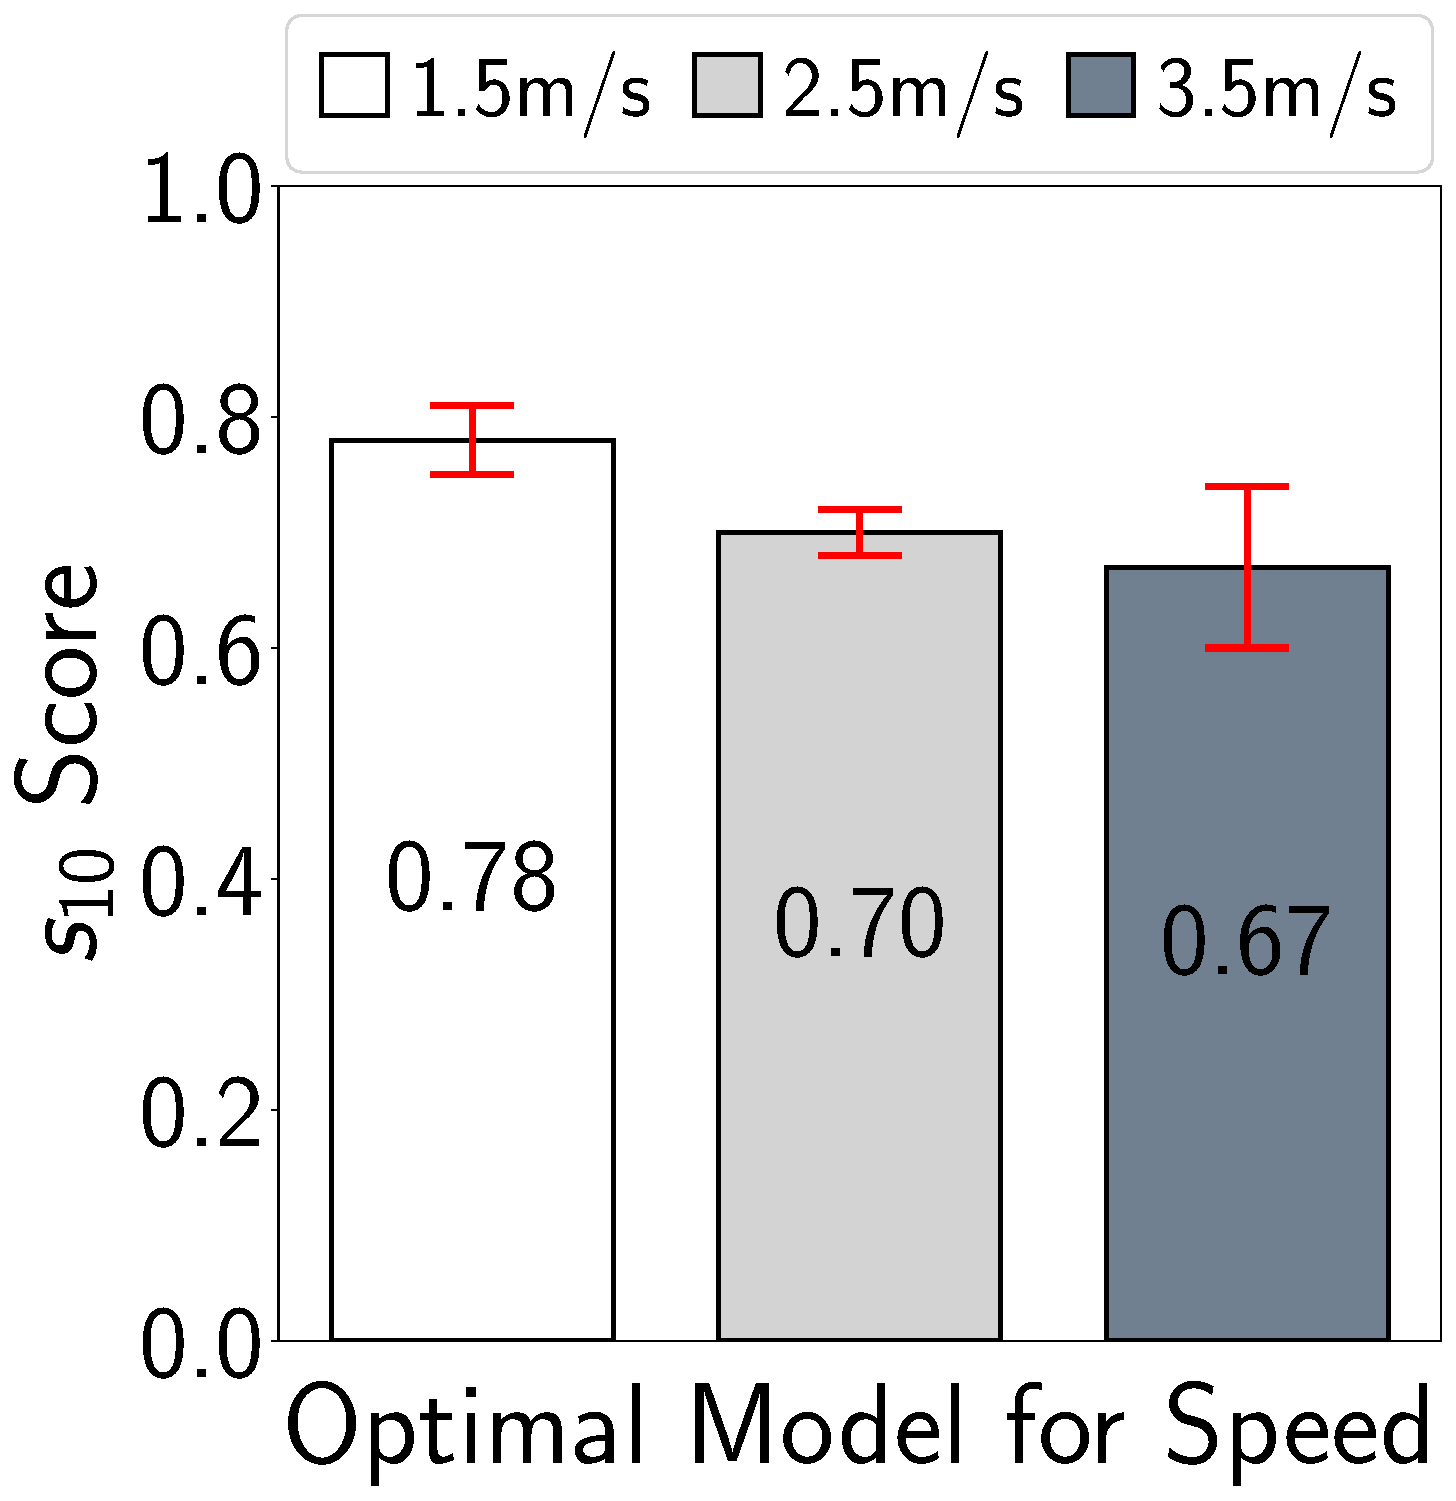
\includegraphics[width=1.0\linewidth]{chapter6/FIGS/fig-tracking-best.pdf}\\
\caption{Baseline Scores}
\label{fig:tracking-best}
\end{minipage}
\begin{minipage}{0.49\linewidth}
\centering
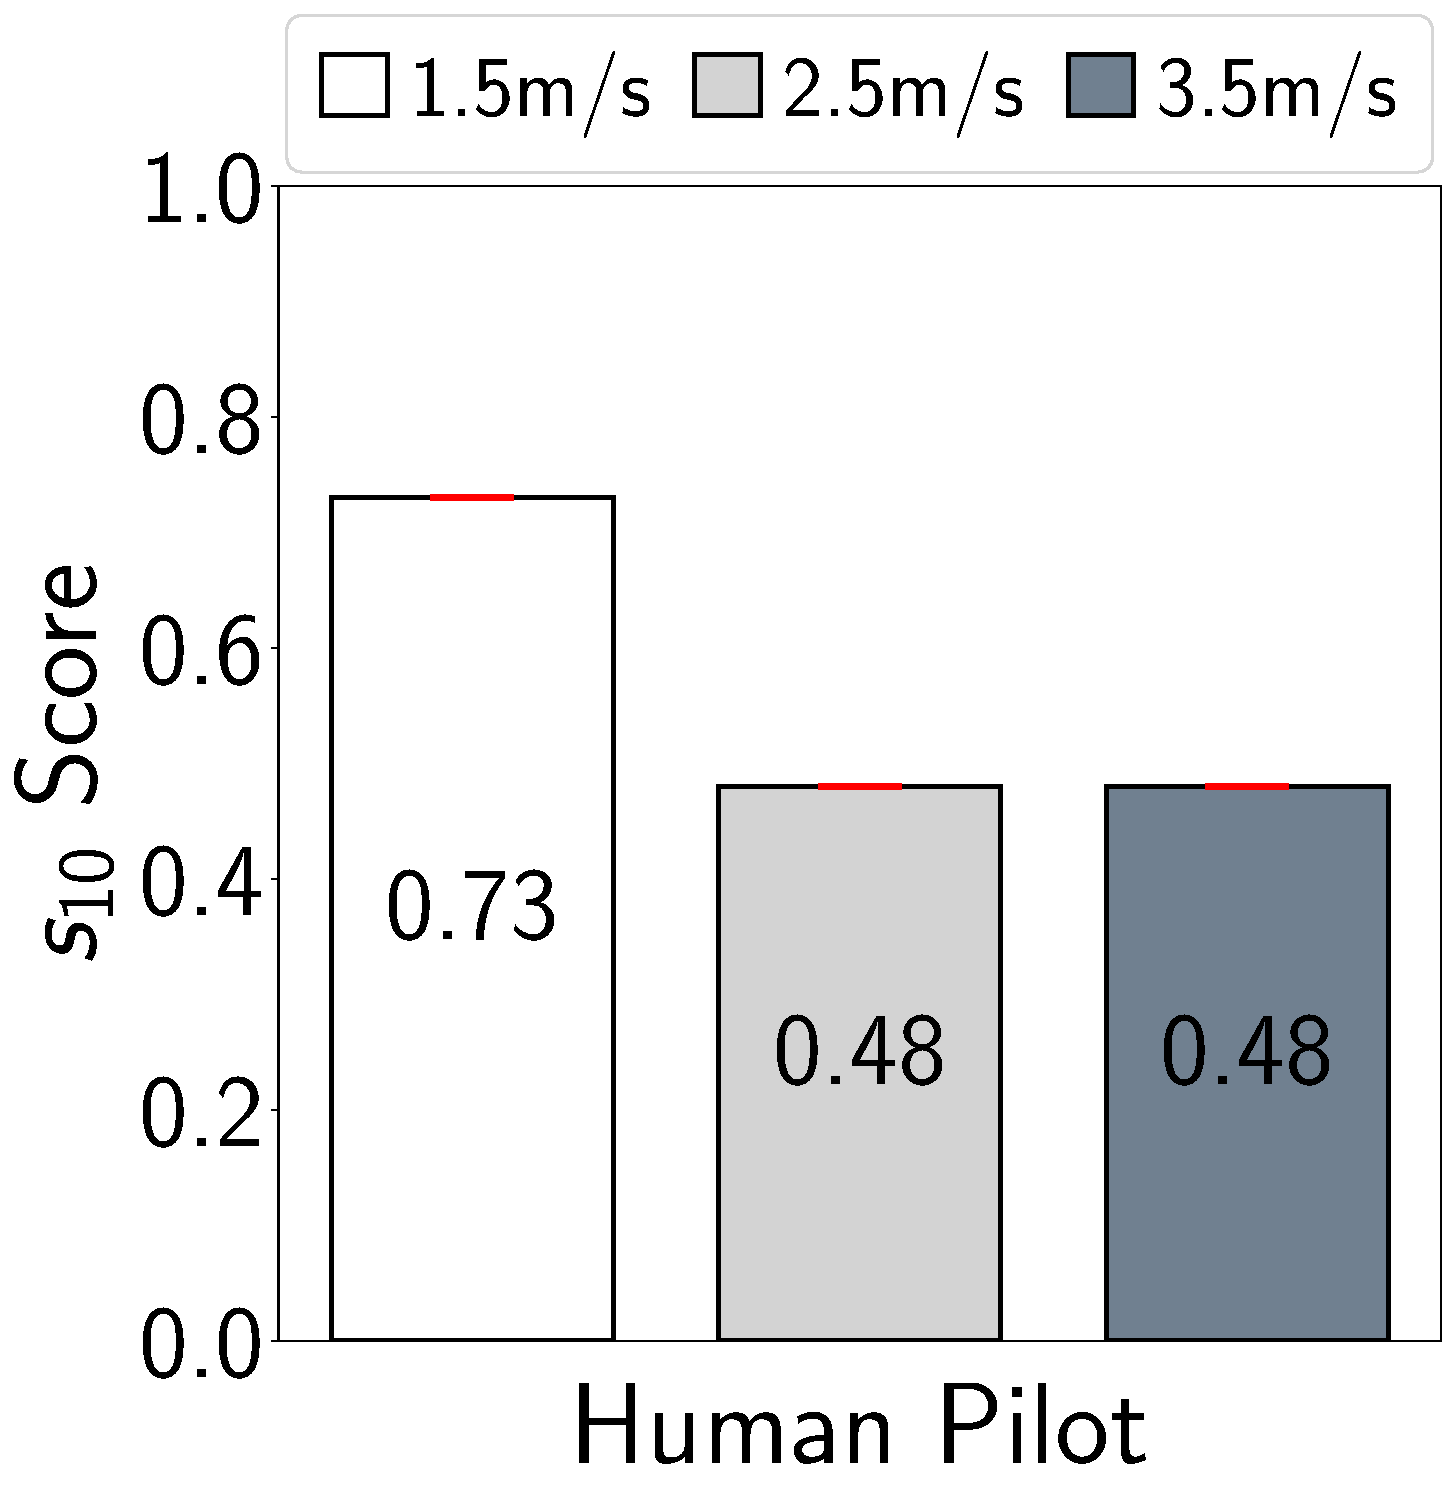
\includegraphics[width=1.0\linewidth]{chapter6/FIGS/fig-tracking-human.pdf}\\
\caption{Human Pilot}
\label{fig:tracking-human}
\end{minipage}
\end{figure}

Since humans are the standard against which AI systems are measured,
I ask how a human pilot does under identical conditions.
To explore this, I manually pilot the drone through the benchmark for the same parameters. I am an experienced pilot on the Parrot Anafi platform with over a dozen hours of flight time. The \ooda~loop is now cyber-human: I uses the drone's live video stream to manually fly it.
Figure~\ref{fig:tracking-human} shows how well I scored
on the benchmark.  Comparing Figures~\ref{fig:tracking-best} and
~\ref{fig:tracking-human}, the autonomous drone and I are comparable at 1.5~m/s, but at higher speeds the autonomous
drone outperforms me. I cannot actuate fast enough to keep up with the rapidly shifting target.

\begin{figure}
\centering
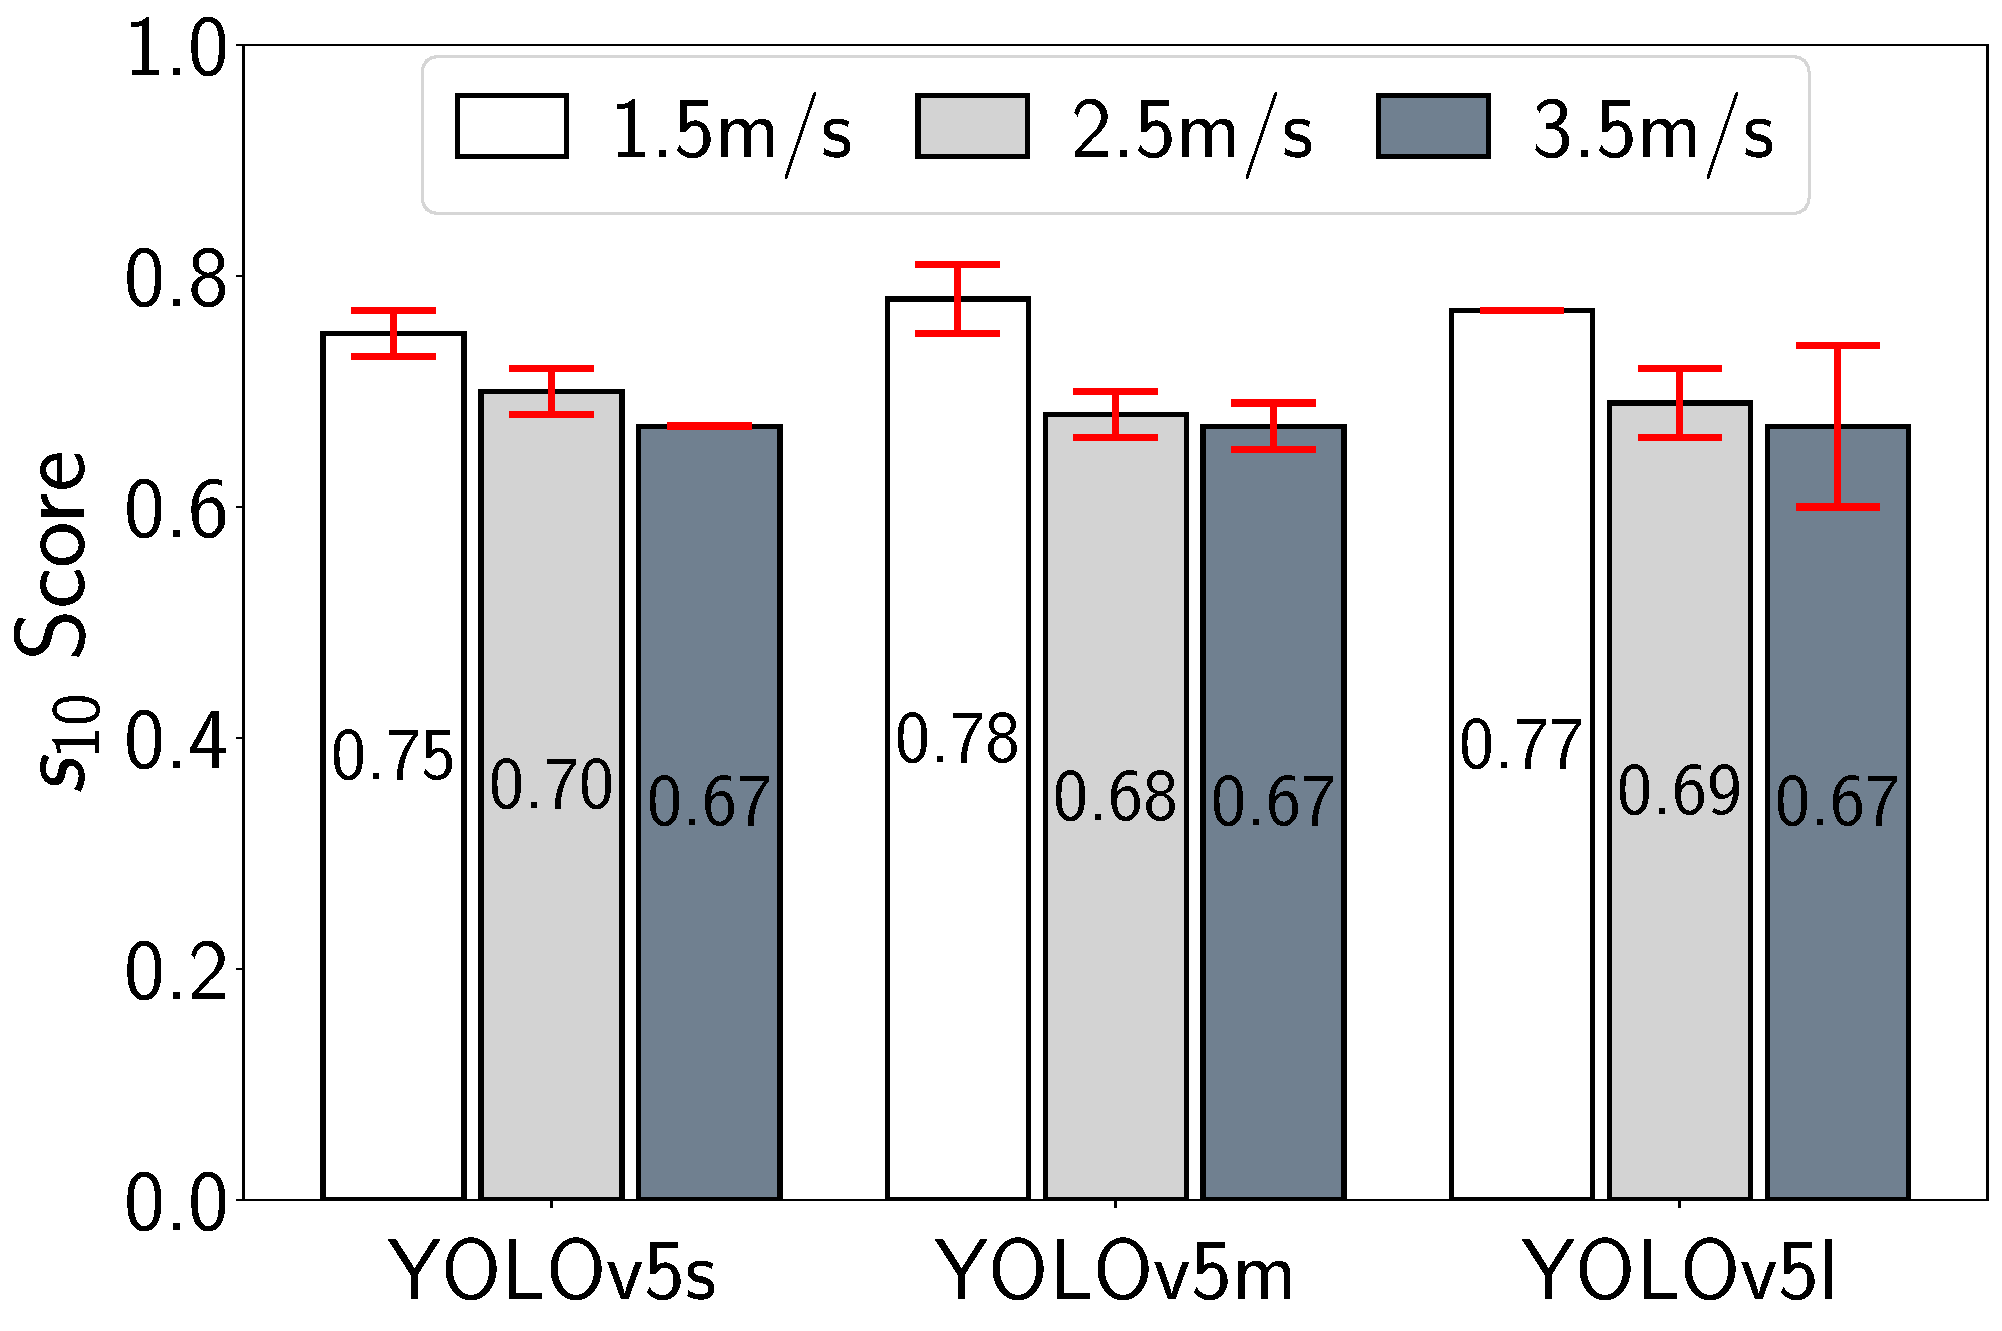
\includegraphics[width=0.8\linewidth]{chapter6/FIGS/fig-tracking-models.pdf}
\caption{\small Impact of YOLO Model on Tracking Benchmark}
\label{fig:track_models}
\end{figure}

\subsection{Impact of Model Accuracy}
\label{sec:tracking-models}

Since multiple DNN models are available to use in
tracking~(Figure~\ref{fig:yolo-model-stats}), I ask the following
question:
\begin{itemize}
\item{\em Does the use of a better model improve tracking?}
\end{itemize}
Figure~\ref{fig:track_models} presents my results.  For any given
speed, there is little difference across models.  The increased
cloudlet load of a more accurate model does not pay off.  However, it
should be noted that this observation may only be true for this
specific tracking benchmark.  As described
in~\S\ref{sec:tracking-description}, the benchmark is defined as being
conducted in an open area free of clutter.  If I were to create a
different tracking benchmark that embodies extensive clutter~(such as
that of a busy street filled with moving cars, bicycles, and
pedestrians, along with static objects such as parked cars and trees),
the results may be quite different. In that case, the improved
accuracy of the larger models may prove decisive. The creation of such a benchmark could be a subject of future work.

\begin{figure}
\centering\small
\begin{minipage}{0.8\linewidth}
\centering
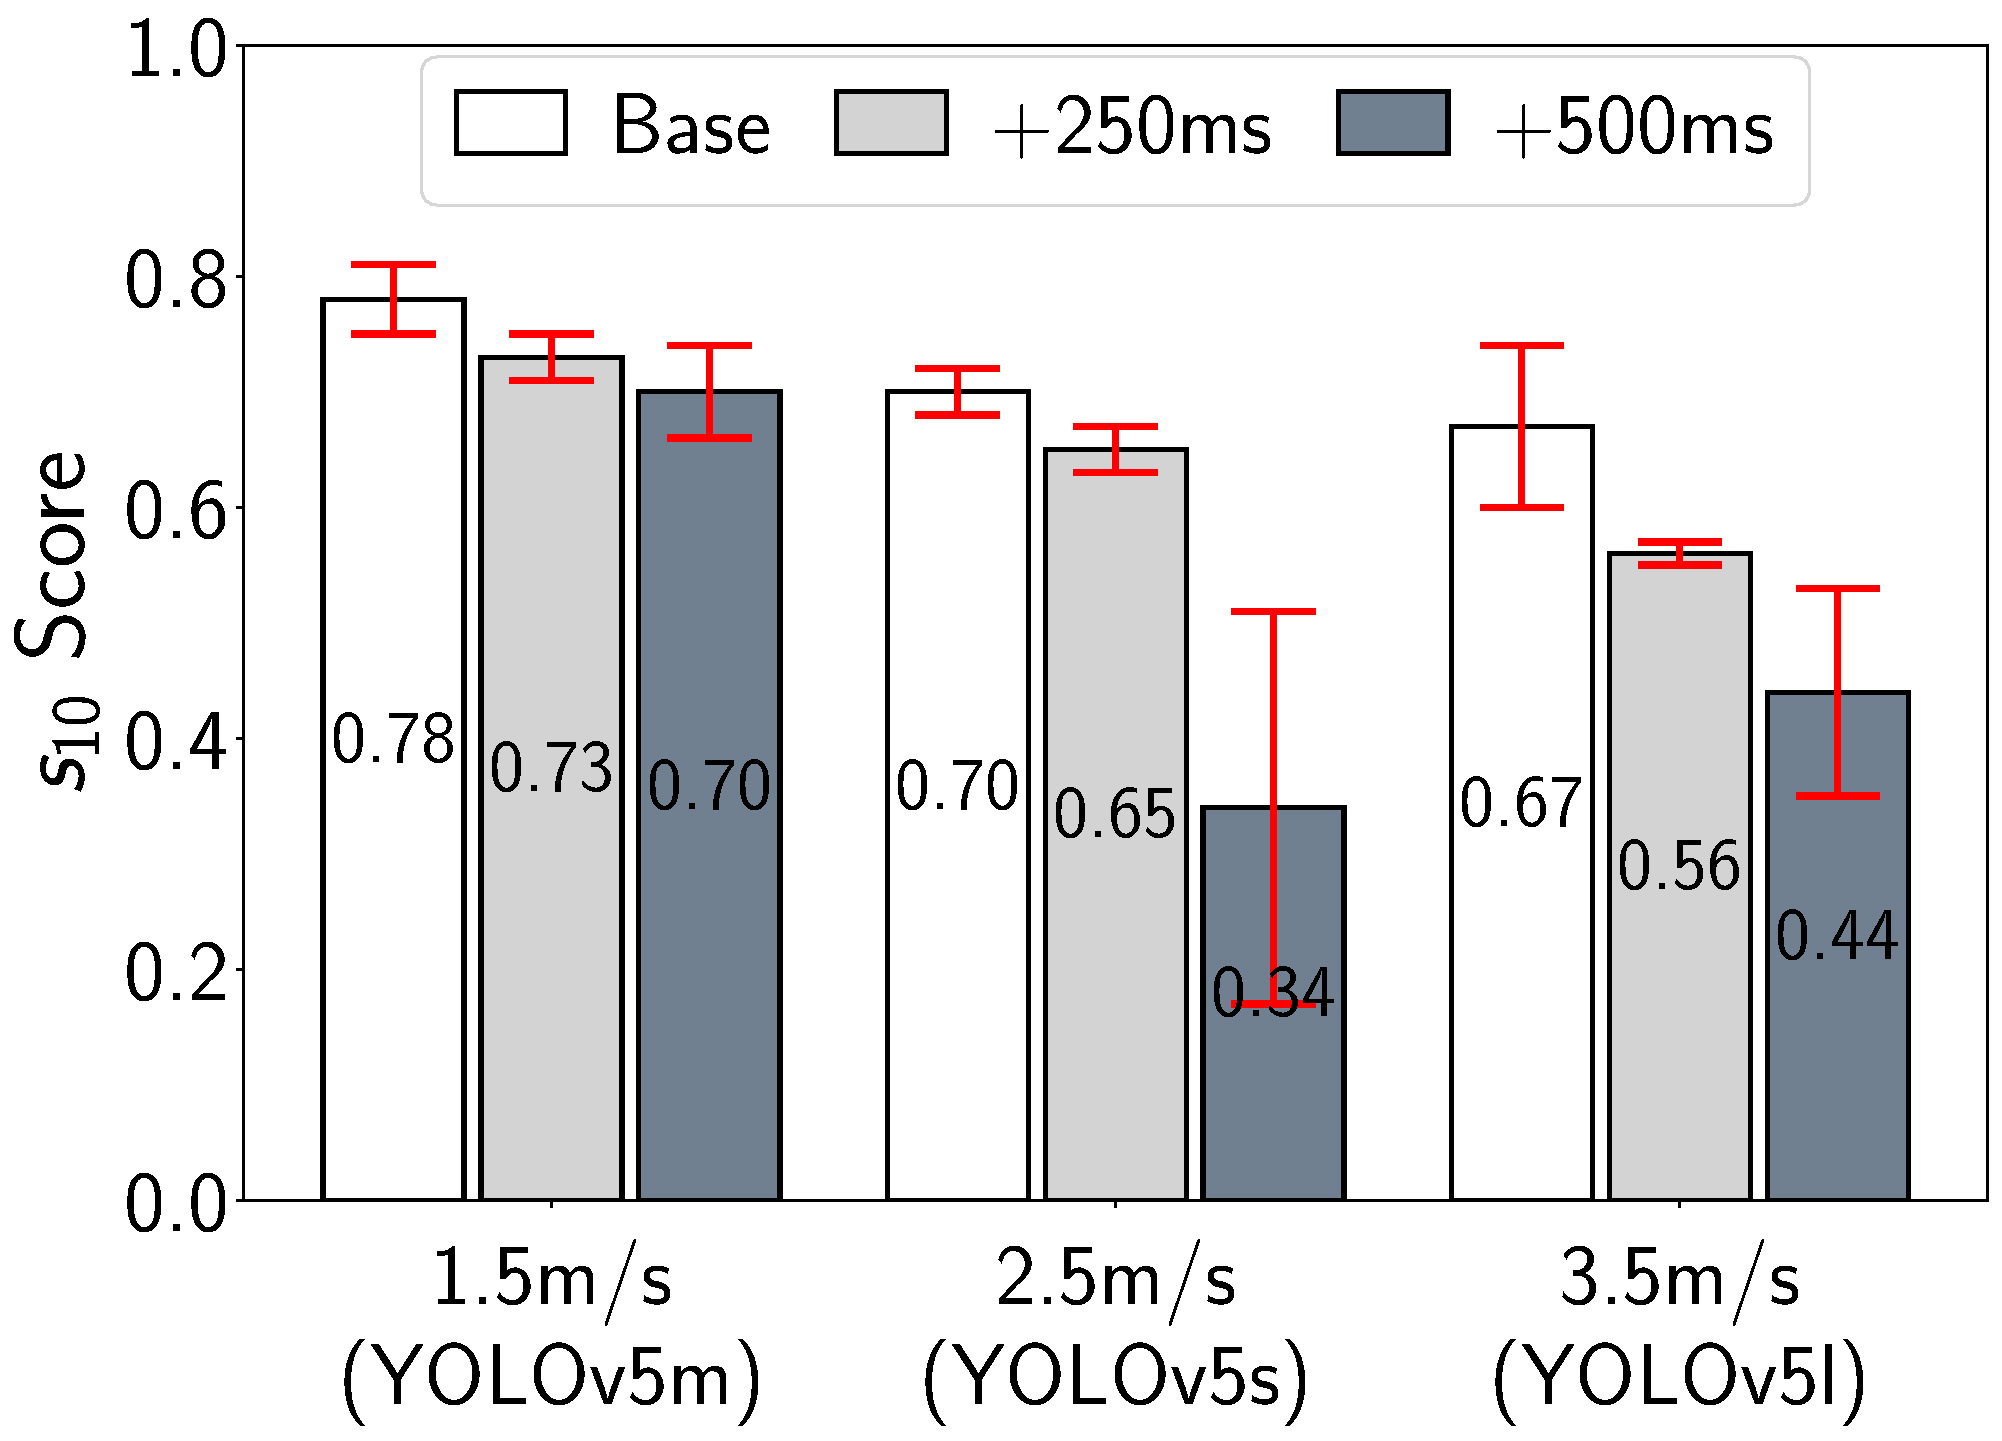
\includegraphics[width=0.98\linewidth]{chapter6/FIGS/fig-tracking-latency.pdf}\\
(a) Additional Latency
\end{minipage}
\begin{minipage}{0.8\linewidth}
\centering
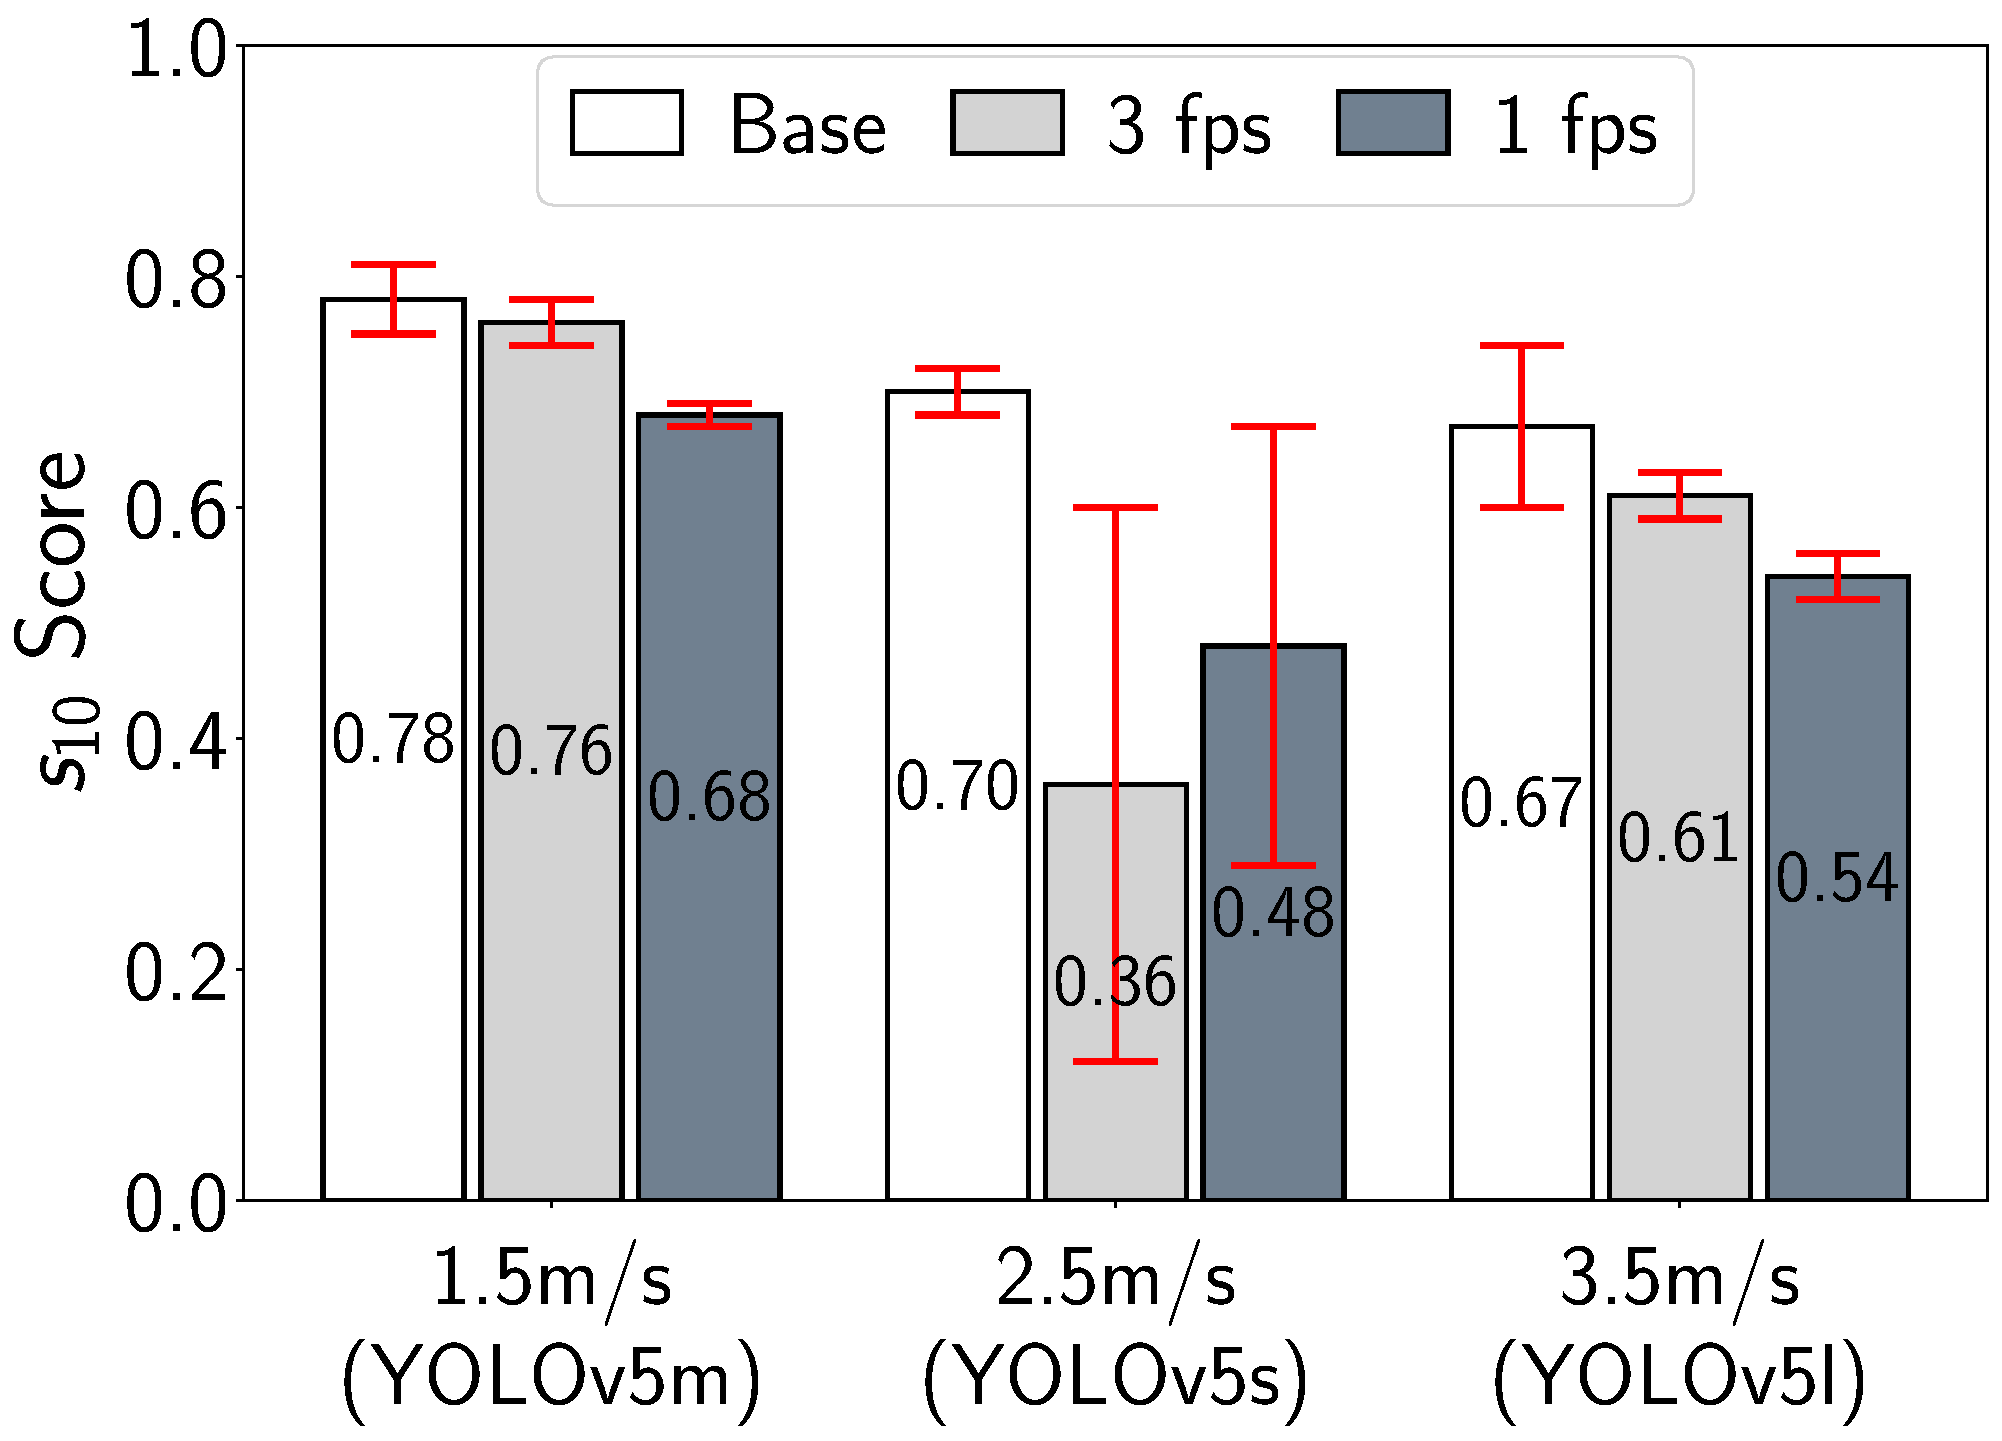
\includegraphics[width=0.98\linewidth]{chapter6/FIGS/fig-tracking-fps.pdf}\\
(b) Reduced Throughput
\end{minipage}
\caption{Impact of Latency and Throughput on Tracking}
\label{fig:tracking-latency-throughput}
\end{figure}

\subsection{Impact of Latency \& Throughput}
\label{sec:tracking-factors}

As in the case of obstacle avoidance~(\S\ref{sec:avoidance-factors}),
I ask:
\begin{itemize}
\item{\em What is the impact of latency or throughput degradation of
    the \ooda~loop on benchmark score?}
\end{itemize}
Figure~\ref{fig:tracking-latency-throughput}(a) shows what happens
when additional latency of 250~ms and 500~ms are added to the
\ooda~loop.  For all target speeds and models, there is a noticeable
drop in benchmark score.  The drop is worse at higher speeds.  This is
directly attributable to the inability of the more sluggish \ooda~loop
to keep the target centered in the FOV.  At higher speeds, the drone
often loses sight of the target early in the tracking.  This results
in a zero score for the remaining frames of that experiment, and hence
an overall low average score.

Figure~\ref{fig:tracking-latency-throughput}(b) shows the same trend
when \ooda~loop throughput is artificially throttled to 3~fps or
1~fps.  At all target speeds and for all models, there is a noticeable
drop in benchmark score.  This drop is greater at higher speeds.

The results in Figures~\ref{fig:tracking-latency-throughput}(a) and
(b) confirm that both end-to-end latency and bottleneck throughput are
important independent factors in determining tracking ability.
Optimizing one at the cost of the other, as occurs when using
strategies such as batching of operations, is unlikely to be
beneficial.

